\section{Exercise 2.1: Creating a Cumulocity IoT Student Account}
So the first was to create a Cumulocity IoT Student Account which might be straight forward but due to 
a outdated exercise description it was not that easy cause the link to the Cumulocity platform was deprecated.
Anyway after finding the way to the Cumulocity IoT page the default dashboard was shown. At this point I am 
not completely sure if there is a need to do this exercise using a new platform or why it is not possible to 
use \code{datacake} which was used in the previous exercise.


\section{Exercise 2.2 Setup}
So setup for this exercise was a real pain an unfortunately the exercise description did not help at all.
The first problem was to even get a working connection to the board via USB to install \code{micropython}.
After installing \code{Thonny} the device were not shown like described further more the 
suggested \code{Arduino Micropython Tools} from Arduino which can be found \href{https://labs.arduino.cc/en}{\textit{here}} 
did not work at all. After some research I found a working solution with \code{Thonny} (see pictures below).
It is highly recommended from my side to update this exercise description and give hints about setting device 
in Bootloader-Mode etc.
\newline
\newline
So the following steps were done to get a working connection to the board:
\begin{enumerate}
  \item Download and install \code{Thonny} from [here](https://thonny.org/)
  \item Open \code{Thonny} and connect the board via USB
  \item Click on \code{Local Python 3} in the upper right corner and select \code{Configure Interpreter}
        \begin{figure}[H]
          \centering
          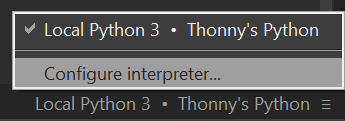
\includegraphics[width=0.6\textwidth]{exercise_micro-python/configure_interpreter.png}
          \caption{Thonny - Configure Interpreter}
        \end{figure}
  \item Select \code{MicroPython(RP2040)} and select the correct port
        \begin{figure}[H]
          \centering
          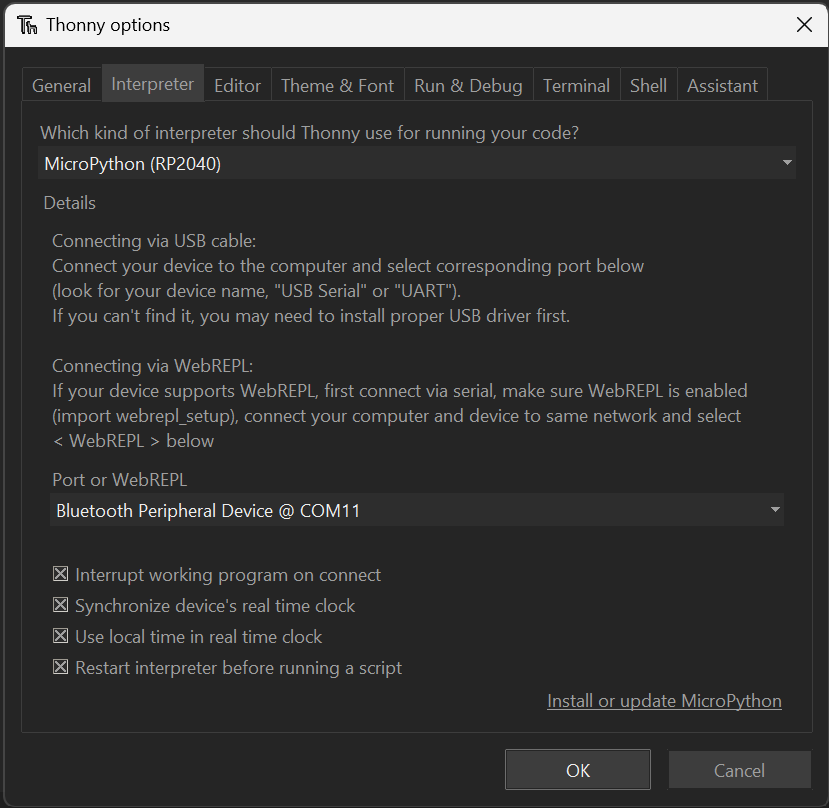
\includegraphics[width=0.6\textwidth]{exercise_micro-python/configure_device.png}
          \caption{Thonny - Select Interpreter}
        \end{figure}
  \item Click on \code{Install or update MicroPython}
  \item Select the target settings like shown in the picture below
        \begin{figure}[H]
          \centering
          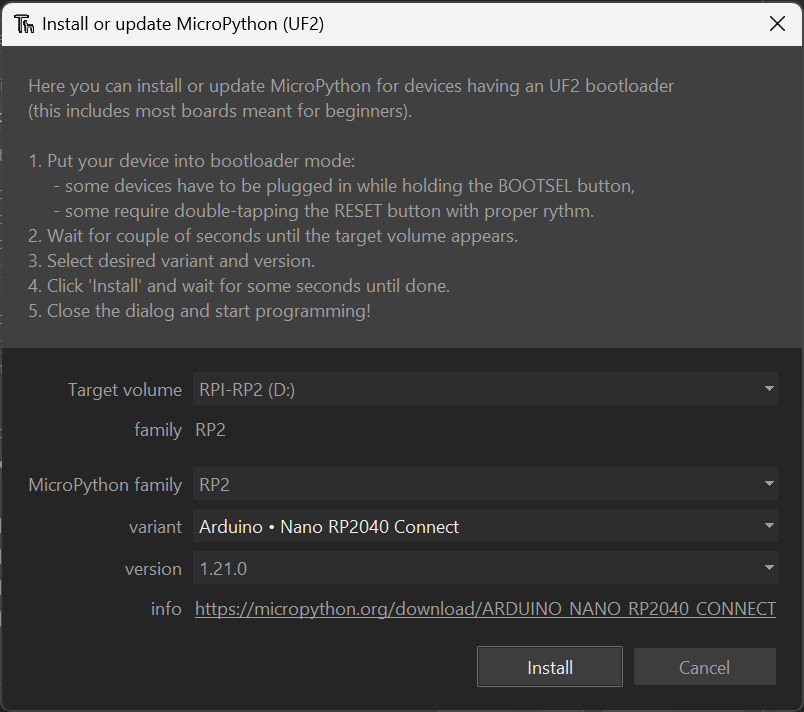
\includegraphics[width=0.6\textwidth]{exercise_micro-python/configure_micro_python.png}
          \caption{Thonny - Install MicroPython}
        \end{figure}
  \item NOTE: In some cases it is necessary to set the board in Bootloader-Mode by pressing \code{Reset} button twice
\end{enumerate}

To test if the installation was successful I used the following code to blink the LED on the board which 
could be found \href{https://forum.arduino.cc/t/blinking-the-rgb-lights-in-micropython/868974}{\textit{here}}:
As this example is very huge I wrote a small script inspired by Arduino page \href{https://docs.arduino.cc/micropython/basics/digital-analog-pins}{\textit{here}}.
The code could be seen bellow, it just blinks the LED connected to PIN 25 on the board.

\begin{minted}
  [
    frame=lines,
    framesep=2mm,
    baselinestretch=1.2,
    linenos
  ]
  {python}
  
  from machine import Pin
  import time

  myLED = Pin(25, Pin.OUT) #Nano RP2040 Connect
  #myLED = Pin(10, Pin.OUT) #Nano 33 BLE / Nano 33 BLE Sense
  #myLED = Pin(2, Pin.OUT) #Portenta H7


  while True:
      print("LED ON")
      myLED.value(0)
      time.sleep(1)
      print("LED OFF")
      myLED.value(1)
      time.sleep(1)
\end{minted}


\subsection{Problem with \code{network} module}

After installing \code{micropython} on the board I tried to connect to the WiFi using the following code which 
could be found \href{https://docs.arduino.cc/micropython/basics/installing-modules}{\textit{here}}:

\begin{minted}
  [
    frame=lines,
    framesep=2mm,
    baselinestretch=1.2,
    linenos
  ]
  {python}
  
  import network

  WIFI_NETWORK='YOUR_NETWORK_NAME'
  WIFI_PASSWORD='YOUR_NETWORK_PASSWORD'

  wlan = network.WLAN(network.STA_IF)
  wlan.active(True)
  wlan.connect(WIFI_NETWORK, WIFI_PASSWORD)

  print()
  print("Connected to ",WIFI_NETWORK)
\end{minted}

This code is also part of the exercise but running this will lead to the following error:

\begin{figure}[H]
  \centering
  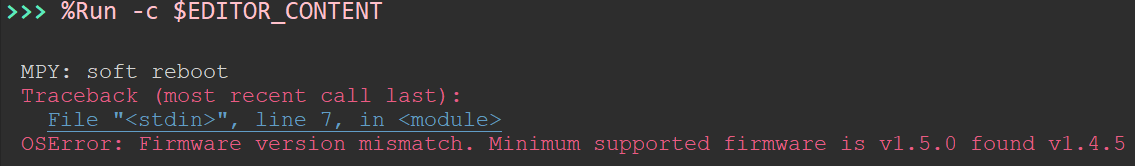
\includegraphics[width=1\textwidth]{exercise_micro-python/network_module_error.png}
  \caption{Error: Network Modul}
\end{figure}

After some research I found out that the \code{network} module is part of the \code{micropython} installation 
and this error is more or less a bug in the \code{micropython} installation. 
Research showed that there is an GitHub issue for this problem which could be found \href{https://github.com/micropython/micropython/issues/8896}{\textit{here}}.
which is still open and the workaround described there is not working for me.
There were several attempts to get this running by flashing the firmware using several tools.
It was flashed using \code{Thonny} and \code{MicroPython Installer} which is a Arduino tool 
which could be found \href{https://labs.arduino.cc/en/labs/micropython-installer/}{\textit{here}}. 
Also it was tested using \code{OpenMV} like described \href{https://docs.arduino.cc/tutorials/nano-rp2040-connect/rp2040-openmv-setup}{\textit{here}}.
Unfortunately none of these attempts were successful and the error still occurs.
Even joining \code{micropythons} Discord channel showed that there is not even a question about this problem.
\newline
\newline
At the end I decided to flash firmware manual to the device like described \href{https://micropython.org/download/ARDUINO_NANO_RP2040_CONNECT/}{\textit{here}}.
This site provides several firmware versions like shown in the image bellow:

\begin{figure}[H]
  \centering
  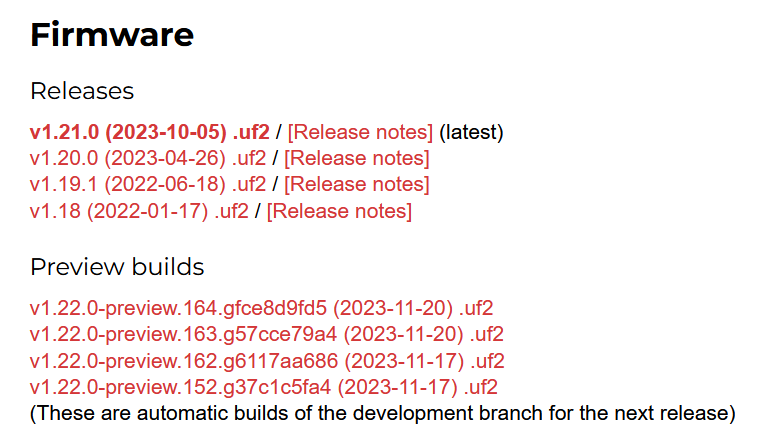
\includegraphics[width=1\textwidth]{exercise_micro-python/firmware_versions.png}
  \caption{Firmware Versions}
\end{figure}

\subsection{Flashing firmware manually}

To flash the firmware manually the following steps were done:
\begin{enumerate}
  \item Download the latest firmware version from \href{https://micropython.org/download/ARDUINO_NANO_RP2040_CONNECT/}{\textit{here}}
  \item Set device in Bootloader-Mode by pressing \code{Reset} button twice. If the device is in Bootloader-Mode the device will open as a new drive like seen bellow:
        \begin{figure}[H]
          \centering
          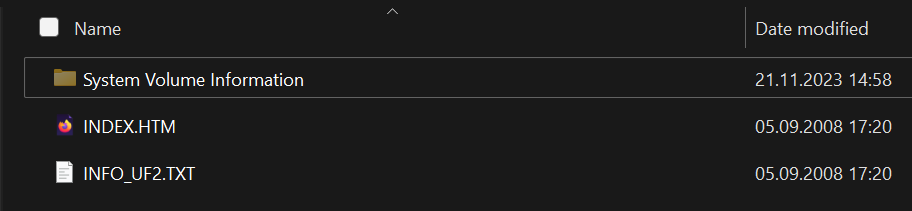
\includegraphics[width=0.6\textwidth]{exercise_micro-python/bootloader_mode.png}
          \caption{Bootloader-Mode}
        \end{figure}
  \item \textbf{Note: } If the device is open as a new drive as shown bellow it is \textbf{NOT} in Bootloader-Mode
        \begin{figure}[H]
          \centering
          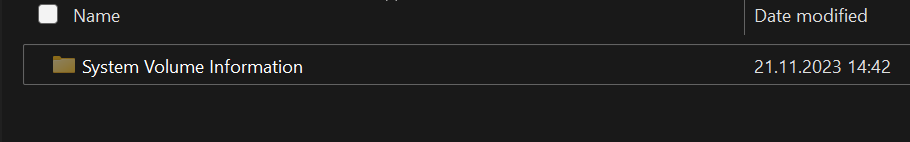
\includegraphics[width=0.6\textwidth]{exercise_micro-python/not_in_bootmode.png}
          \caption{Bootloader-Mode}
          \label{fig:no_bootloader_mode}
        \end{figure}
  \item Copy the downloaded firmware to the devices root folder
  \item After copying the firmware the device will reboot and the firmware will be flashed
  \item After flashing the device will open as a new drive again like seen in figure \ref{fig:no_bootloader_mode}
  \item When opening the device in e.g. \code{Thonny} the current firmware version will be shown in the shell
\end{enumerate}

All released firmware were tested as well as one preview version.
When flashing \textbf{v1.18} the device will not show up as a drive and there is still a warning about 
firmware mismatching but no error when running. This was the only version which did not show the error.

\subsection{Updating Arduino Firmware}

After more testing i figured out that there are more errors when using micropython on an Arudino board 
which has a firmware version lower than \textbf{1.4.8} installed (so unfortunately this is no official information 
but was posted on Arduino forum and after struggling with it for a few hours, I can confirm this).
\newline
\newline
So updating the firmware would be a easy one cause it can be done using the Arduino IDE.
Guess what, this was not working as well. Cause there was micropython flashed to the board the Arduino IDE 
was not able to upload scripts or update the firmware. Don't know exactly what i did but after 
pressing BOOTLOADER button and flashing several micropython versions once it was possible to upload 
sketches from Arduino IDE again. After that it was possible to update the firmware using the Arduino IDE 
which can be seen in the picture bellow:
\begin{figure}[H]
  \centering
  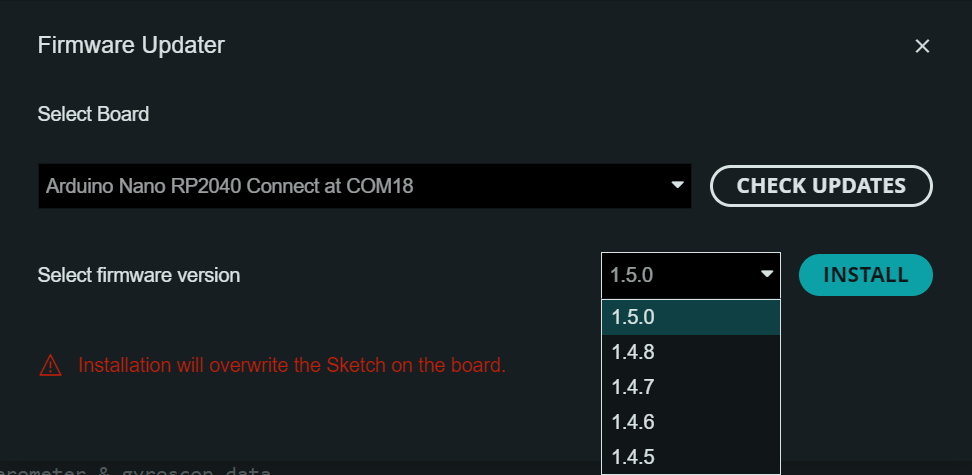
\includegraphics[width=0.8\textwidth]{exercise_micro-python/update_firmware.png}
  \caption{Update Firmware}
\end{figure}

\subsection{Using WiFi with \code{micropython}}

After this long journey (in which I unfortunately did not fight a dragon in a mountain full of gold 
and thus helped a dwarf tribe to freedom). It was possible to connect to the WiFi using the code 
shown above resulting in the following output:

\begin{figure}[H]
  \centering
  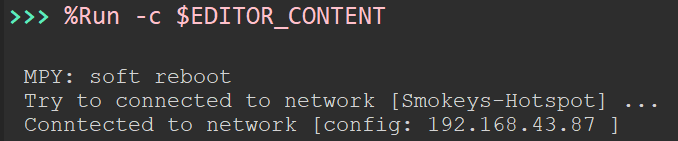
\includegraphics[width=1\textwidth]{exercise_micro-python/wifi_connected.png}
  \caption{WiFi Connected}
\end{figure}

\section{Sending data from the Arduino to Cumulocity IoT}

The last exercise was to send data from the Arduino to Cumulocity IoT. This was done using the code 
shown in \code{main.py} of the repository which could be found \href{https://github.com/Smokey95/AIN_Ubiquitous_Computing/tree/main/exercise/sheet%202}{\textit{here}}.
Cause the code is very huge I will not post it here but it is well documented and should be self-explanatory.
\newline
\newline
For this exercise it would also be required to access the sensors on the board.
Access the boards sensors was done using the \code{LSM6DSOX} library and the code 
provided \href{https://micropython-lsm6dsox.readthedocs.io/en/latest/examples.html}{\textit{here}}.
\textbf{Note:} The \code{SDA} and \code{SCL} pins are different on the Arduino board and has to 
be changed like shown \href{https://docs.arduino.cc/tutorials/nano-rp2040-connect/rp2040-openmv-mlc}{\textit{here}}.
To import the library i wrote a small script \code{import\_lsm6dsox.py} which imports the library using \code{mip}.
\newline
\newline
After setting up everything it was possible to send data to Cumulocity IoT resulting in the following output:
\begin{figure}[H]
  \centering
  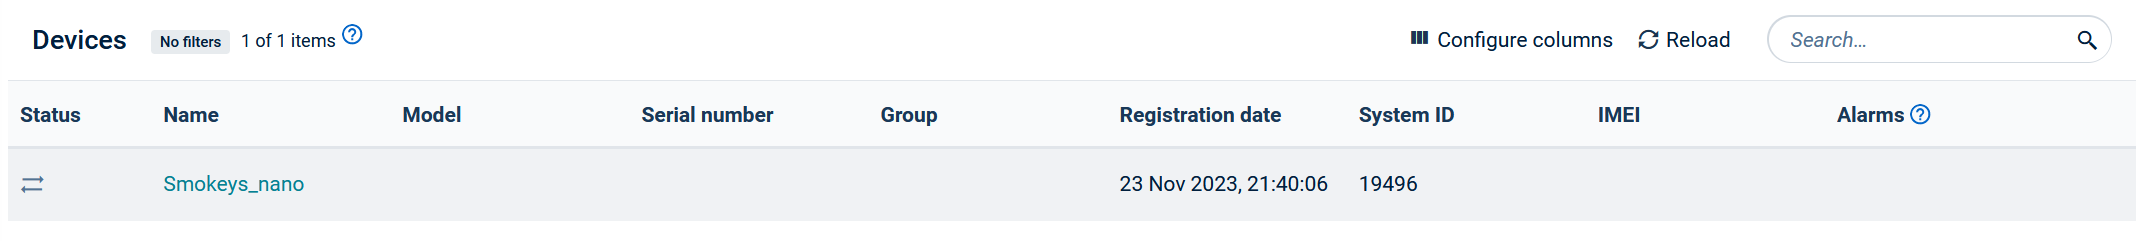
\includegraphics[width=1\textwidth]{exercise_micro-python/send_data.png}
  \caption{Send Data}
\end{figure}